% Created 2024-04-04 Thu 13:51
% Intended LaTeX compiler: pdflatex
\documentclass[11pt]{article}
\usepackage[utf8]{inputenc}
\usepackage[T1]{fontenc}
\usepackage{graphicx}
\usepackage{longtable}
\usepackage{wrapfig}
\usepackage{rotating}
\usepackage[normalem]{ulem}
\usepackage{amsmath}
\usepackage{amssymb}
\usepackage{capt-of}
\usepackage{hyperref}
\usepackage{listings}
\usepackage{color}
\usepackage{amsmath}
\usepackage{array}
\usepackage[T1]{fontenc}
\usepackage{natbib}
\author{Anders Munch}
\date{\today}
\title{}
\begin{document}

\tableofcontents

Remember to exceture (C-c C-c) the following line:


\section{Packages and setup}
\label{sec:org3001f1d}
\#+RESULTS[(2023-07-10 09:28:28) a2b10d472d503e2facd58b5fa9ea661e3dc33409]:


\section{sandbox}
\label{sec:org1104cd8}
\#+RESULTS[(2024-04-03 12:10:39) fee665afcd6283305bb47ea7788468cc4d229ad4]:


\section{Hold-out sample problem}
\label{sec:org4240dec}
\begin{center}
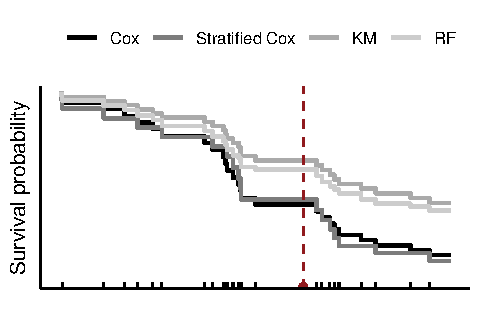
\includegraphics[width=.9\linewidth]{sl-hold-out-sample.pdf}
\end{center}



\section{IPCW circel}
\label{sec:orgafe3f90}

\begin{center}
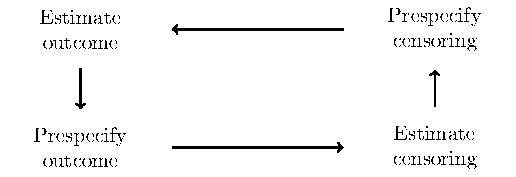
\includegraphics[width=.9\linewidth]{ipcw-circle.pdf}
\end{center}

\section{Censoring and multi-state system}
\label{sec:orgf298cfb}

\begin{center}
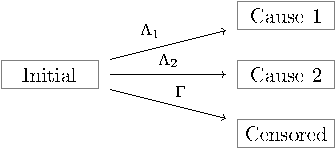
\includegraphics[width=.9\linewidth]{comp-risk-observed-w-text.pdf}
\end{center}

\begin{center}
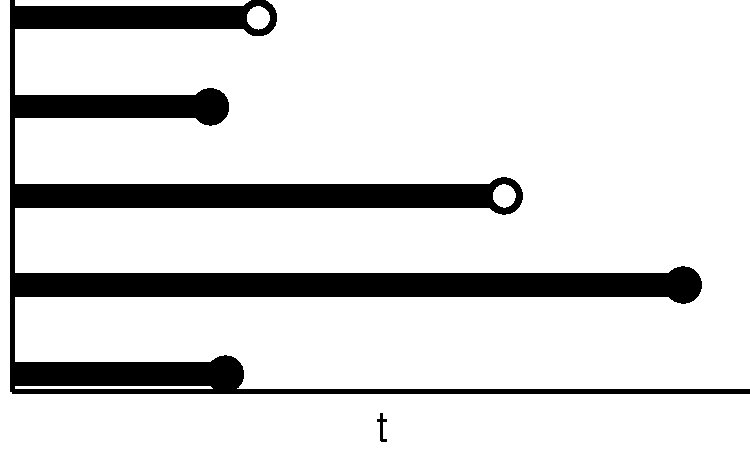
\includegraphics[width=.9\linewidth]{./multi-state-data-1.pdf}
\end{center}

\begin{center}
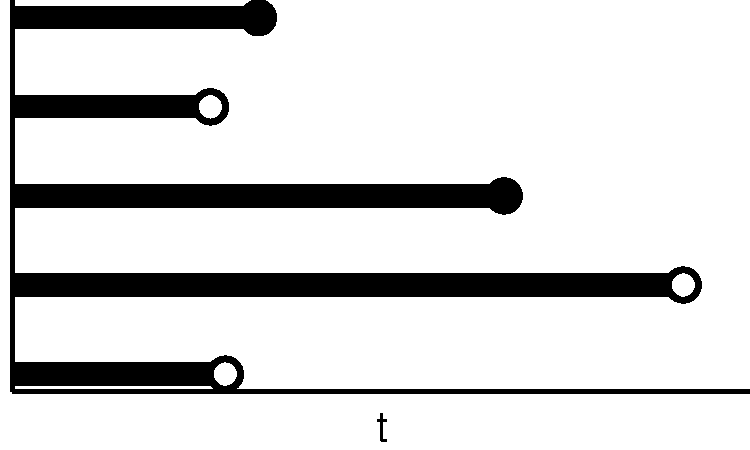
\includegraphics[width=.9\linewidth]{./multi-state-data-2.pdf}
\end{center}

\begin{center}
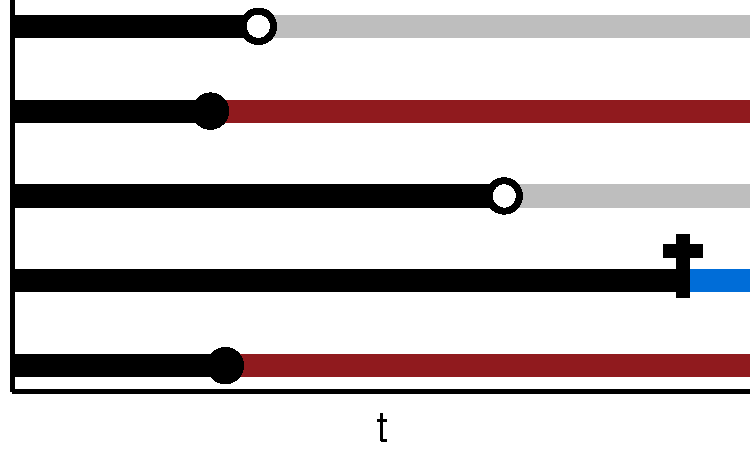
\includegraphics[width=.9\linewidth]{./multi-state-data-3.pdf}
\end{center}

\section{Illustration zelefsky data}
\label{sec:orga70ad2a}

\begin{center}
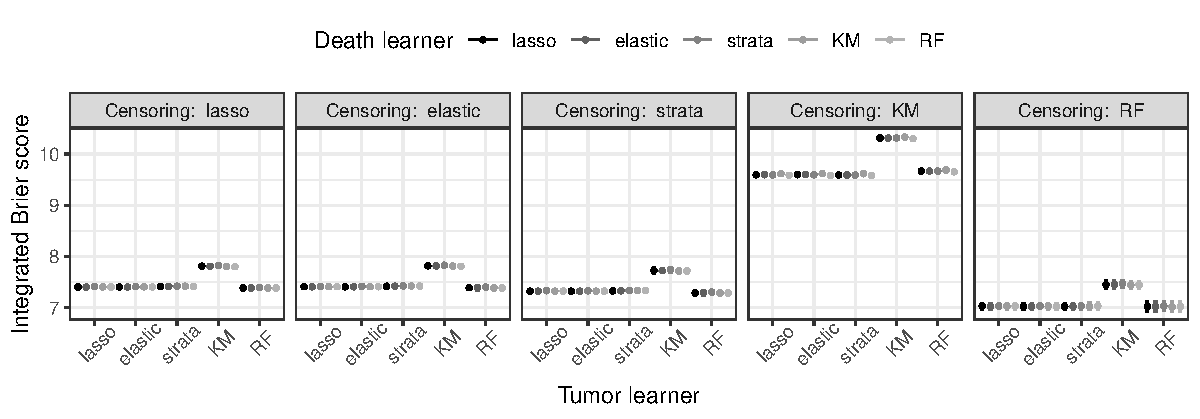
\includegraphics[width=.9\linewidth]{zelefski-real-data.pdf}
\end{center}

\begin{verbatim}
     cause1  cause2 censor      loss
  1:     RF      KM     RF  7.022057
  2: strata elastic     RF  7.025097
  3:     RF elastic     RF  7.025267
  4:     RF      RF     RF  7.025504
  5: strata   lasso     RF  7.025648
 ---                                
121:     KM      RF     KM 10.299304
122:     KM   lasso     KM 10.310004
123:     KM elastic     KM 10.310062
124:     KM  strata     KM 10.310763
125:     KM      KM     KM 10.328653
\end{verbatim}
\end{document}